\documentclass{article}
\usepackage{ae,aecompl}
\usepackage{todonotes}
\usepackage{chngcntr}
\usepackage{tikz-cd}
\usepackage{graphicx}
\graphicspath{ {./images/}}
\usepackage[all,cmtip]{xy}
\usepackage{amsmath, amscd}
\usepackage{amsthm}
\usepackage{amssymb}
\usepackage{amsfonts}
\usepackage{bm}
\usepackage{qsymbols}
\usepackage{latexsym}
\usepackage{mathrsfs}
\usepackage{mathtools}
\usepackage{cite}
\usepackage{color}
\usepackage{url}
\usepackage{enumerate}
\usepackage{verbatim}
\usepackage[draft=false, colorlinks=true]{hyperref}
\usepackage{pdfpages}
\usepackage[margin=1.2in]{geometry}
\usepackage{IEEEtrantools}

\usepackage{fancyhdr}


\usepackage[nameinlink]{cleveref}


\DeclareMathOperator*{\ac}{accept}
\DeclareMathOperator*{\amax}{argmax}
\DeclareMathOperator*{\amin}{argmin}
\DeclareMathOperator*{\Aut}{Aut}
\newcommand {\al}{{\alpha}}
\newcommand {\abs}[1]{{\left\lvert#1\right\rvert}}
\newcommand {\A}{{\mathcal{A}}}
\newcommand {\AM}{{\mathrm{AM}}}
\newcommand {\AMp}{{\AM_{p}^{X}\!(\Ri_\w)}}
\newcommand {\B}{{\mathcal{B}}}
\DeclareMathOperator*{\Be}{Bern}
\newcommand {\Br}{{\dot{B}}}
\newcommand {\Ba}{{\mathfrak{B}}}
\newcommand {\C}{{\mathbb C}}
\newcommand {\ce}{\mathrm{c}}
\newcommand {\Ce}{\mathrm{C}}
\newcommand {\Cc}{\mathrm{C_{c}}}
\newcommand {\Ccinf}{\mathrm{C_{c}^{\infty}}}
\DeclareMathOperator{\cov}{Cov}
\DeclareMathOperator{\DEV}{DEV}
\newcommand {\Di}{{\mathbb D}}
\newcommand {\dom}{\mathrm{dom}}
\newcommand{\dist}{\stackrel{\mathrm{dist}}{=}}
\newcommand {\ud}{\mathrm{d}}
\newcommand {\ue}{\mathrm{e}}
\newcommand {\eps}{\varepsilon}
\newcommand {\veps}{\varepsilon}
\newcommand {\vrho}{{\varrho}}
\newcommand {\E}{{\mathbb{E}}}
\newcommand {\Ec}{{\mathcal{E}}}
\newcommand {\Ell}{L}
\newcommand {\Ellp}{{L_{p}[0,1]}}
\newcommand {\Ellpprime}{{L_{p'}([0,1])}}
\newcommand {\Ellq}{{L_{q}([0,1])}}
\newcommand {\Ellqprime}{{L_{q'}([0,1])}}
\newcommand {\Ellr}{L^{r}}
\newcommand {\Ellone}{{L_{1}([0,1])}}
\newcommand{\Elltwo}{{L_{2}([0,1])}}
\newcommand{\Ellinfty}{L^{\infty}}
\newcommand{\Ellinftyc}{L_{\mathrm{c}}^{\infty}}
\newcommand{\exb}[1]{\exp\left\{#1\right\}}
\DeclareMathOperator*{\Ext}{Ext}
\newcommand{\F}{{\mathcal{F}}}
\newcommand{\Fe}{{\mathbb{F}}}
\newcommand{\G}{{\mathcal{G}}}
\newcommand{\HF}{\mathcal{H}_{\text{FIO}}^{1}(\Rd)}
\newcommand{\Hr}{H}
\newcommand{\HT}{\mathcal{H}}
\newcommand{\ui}{\mathrm{i}}
\newcommand{\I}{{I}}
\newcommand{\J}{{\mathcal{J}}}
\newcommand{\id}{{\mathrm{id}}}
\newcommand{\iid}{\stackrel{\mathclap{\normalfont\mbox{iid}}}{\sim}}
\newcommand{\im}{{\text{im }}}
\newcommand{\ind}{{\perp\!\!\!\perp}}
\DeclareMathOperator*{\Int}{int}
\newcommand{\intx}{{\overline{\int_{X}}}}
\newcommand{\inte}{{\overline{\int_{\E}}}}
\newcommand{\la}{\lambda}
\newcommand{\rb}{\rangle}
\newcommand{\lb}{{\langle}}
\newcommand{\La}{\Lambda}
\newcommand{\calL}{{\mathcal{L}}}
\newcommand{\lp}{{\mathcal{L}}^{p}}
\newcommand{\lpo}{{\overline{\mathcal{L}}^{p}\!}}
\newcommand{\Lpo}{{\overline{\Ell}^{p}\!}}
\newcommand{\M}{{\mathbf{M}}}
\newcommand{\Ma}{{\mathcal{M}}}
\newcommand{\N}{{{\mathbb N}}}
\newcommand{\Na}{{{\mathcal{N}}}}
\newcommand{\norm}[1]{\left\|#1\right\|}
\newcommand{\normm}[1]{{\left\vert\kern-0.25ex\left\vert\kern-0.25ex\left\vert #1 
    \right\vert\kern-0.25ex\right\vert\kern-0.25ex\right\vert}}
\newcommand{\Om}{{{\Omega}}}
\newcommand{\one}{{{\bf 1}}}
\newcommand{\pic}{\text{Pic }}
\newcommand{\ph}{{\varphi}}
\newcommand{\Pa}{{\mathbb{P}}}
\newcommand{\Po}{{\mathcal{P}}}
\newcommand{\Q}{{\mathbb{Q}}}
\newcommand{\R}{{\mathbb R}}
\newcommand{\Rd}{{\mathbb{R}^{d}}}
\DeclareMathOperator{\rej}{reject }
\newcommand{\Rn}{{\mathbb{R}^{n}}}
\newcommand{\cR}{{\mathcal{R}}}
\newcommand{\Rad}{{\mathrm{Rad}}}
\newcommand{\ran}{{\mathrm{ran}}}
\newcommand{\Ri}{{\mathrm{R}}}
\newcommand{\supp}{{\mathrm{supp}}}
\newcommand{\Se}{\mathrm{S}}
\newcommand{\Sp}{S^{*}(\Rn)}
\newcommand{\St}{{\mathrm{St}}}
\newcommand{\Sw}{\mathcal{S}}
\newcommand{\T}{{\mathcal{T}}}
\newcommand{\ta}{{\theta}}
\newcommand{\Ta}{{\Theta}}
\newcommand{\topp}{\stackrel{p}{\to}}
\newcommand{\todd}{\stackrel{d}{\to}}
\newcommand{\toL}[1]{\stackrel{L^{#1}}{\to}} 
\newcommand{\toas}{\stackrel{a.s.}{\to}}
\DeclareMathOperator{\V}{Var}
\newcommand {\w}{{\omega}}
\newcommand {\W}{{\mathrm{W}}}
\newcommand {\Wnp}{\text{$\mathrm{W}$\textsuperscript{$n,\!p$}}}
\newcommand {\Wnpeq}{\text{$\mathrm{W}$\textsuperscript{$n\!,\!p$}}}
\newcommand {\Wonep}{\text{$\mathrm{W}$\textsuperscript{$1,\!p$}}}
\newcommand {\Wonepeq}{\text{$\mathrm{W}$\textsuperscript{$1\!,\!p$}}}
\newcommand {\X}{{\mathcal{X}}}
\newcommand {\Z}{{{\mathbb Z}}}
\newcommand {\Za}{{\mathcal{Z}}}
\newcommand {\Zd}{{\Z[\sqrt{d}]}}
\newcommand {\vanish}[1]{\relax}

\newcommand {\wh}{\widehat}
\newcommand {\wt}{\widetilde}
\newcommand {\red}{\color{red}}

% Distributions
\newcommand{\normal}{\mathsf{N}}
\newcommand{\poi}{\mathsf{Poisson}}
\newcommand{\bern}{\mathsf{Bernoulli}}
\newcommand{\bin}{\mathsf{Binomal}}
\newcommand{\multi}{\mathsf{Multinomial}}
\newcommand{\Exp}{\mathsf{Exp}}



% put your command and environment definitions here




% some theorem environments
% remove "[theorem]" if you do not want them to use the same number sequence


  \newtheorem{thrm}{Theorem}
  \newtheorem{lemma}{Lemma}
  \newtheorem{prop}{Proposition}
  \newtheorem{cor}{Corollary}

  \newtheorem{conj}{Conjecture}
  \renewcommand{\theconj}{\Alph{conj}}  % numbered A, B, C etc

  \theoremstyle{definition}
  \newtheorem{defn}{Definition}
  \newtheorem{ex}{Example}
  \newtheorem{exs}{Examples}
  \newtheorem{question}{Question}
  \newtheorem{remark}{Remark}
  \newtheorem{notn}{Notation}
  \newtheorem{exer}{Exercise}




\title{STATS305A - Lecture 5}
\author{John Duchi\\ Scribed by Michael Howes}
\date{05/10/21}

\pagestyle{fancy}
\fancyhf{}
\rhead{STATS305A - Lecture 5}
\lhead{05/10/21}

\begin{document}
\maketitle
\tableofcontents
\section{Announcements}
\begin{itemize}
    \item John's office hours will be after class 11:15-12. Tuesdays and Thursdays.
    \item Homework 1 is due on Friday. There is an extra coding question which was added this weekend.
    \item Etude coming on Friday.
    \item Data for coding questions is available on website unless otherwise stated.
    \item Course notes from last week to be uploaded soon.
\end{itemize}
\section{Inference}
We want to know if various parameters in our model ``matter''. We will design tests that ask this question. Recall that we have
\begin{thrm}
    If $Y=X\beta + \varepsilon$ and $\varepsilon \sim \Na(0, \sigma^2 I)$, then (key independenc results)
    \begin{enumerate}
        \item $\wh{\beta} = (X^TX)^{-1}X^Y \sim \Na(\beta, (X^TX)^{-1})$.
        \item $\wh{Y}=X\wh{\beta} = HY \sim \Na(X\beta,\sigma^2 H)$.
        \item $\wh{\varepsilon} = (I-H)Y = (I-H)\varepsilon \sim \Na(0, \sigma^2(I-H))$.
        \item $\wh{\varepsilon} \ind (\wh{\beta},\wh{Y})$.
    \end{enumerate}
    where $H = X(X^TX)^{-1}X$ is the projection onto the range of $X$.
\end{thrm}
\subsection{Testing linear functionals}
Say we are curious about the value of $c^T\beta$ where $c \in \R^d$. A common example is when $c = e_j$ ($j^{th}$ basis vector), then $c^T\beta = e_j^T\beta = \beta_j$.

By our key independence result we have
\[c^T(\wh{\beta}-\beta) \sim \Na(0, \sigma^2 c^T(X^TX)^{-1}c), \]
and
\begin{IEEEeqnarray*}{rCl}
    S^2 &:= &\frac{1}{n-d}\norm{\wh{\varepsilon}}_2^2\\
    &=& \frac{1}{n-d}\sum_{i=1}^n (x_i^T\beta - Y_i)^2\\
    &=&\frac{1}{n-d}\norm{(I-H)\varepsilon}_2^2\\
    &\sim& \frac{\sigma^2}{n-d} \chi^2_{n-d}.
\end{IEEEeqnarray*}
Since $I-H$ has rank $n-d$. We alos have $S^2 \ind (\wh{\beta}-\beta)$ and thus
\[\frac{c^T(\wh{\beta}-\beta)}{s\sqrt{c^T(X^TX)^{-1}}} \sim T_{n-d}. \]
This gives us the t-test.
\subsection{T-test of significance}
Assume $c^T\beta =0$ (this is our null hypothesis, $H_0$). Reject the null if 
\[t:= \frac{c^T\wh{\beta}}{S\sqrt{c^T(X^TX)^{-1}C}}, \]
is far from 0. 

In the \underline{two sided T-test} our $p$-value is 
\[\Pa(\abs{T_{n-d}}\ge \abs{t}), \]
and we reject the null if this value is small.

In the \underline{one sided T-test} we only care if $c^T\beta \ge 0$. In which case our $p$-value if
\[\Pa(T_{n-d} \ge t), \]
and we again reject the null if this value is small. 

\begin{ex}
    Suppose we are doing drug development and we have 
    \[X_i := \begin{cases}
        1 & \text{if person } i \text{ received treatment},\\
        0 &\text{ otherwise}.
    \end{cases} \]
    and $Y=$ survival time. We will then have the model $Y = \beta_0 + \beta_1 X + \varepsilon$. We are interested in whether or $\beta_1 \ge 0$. Thus we will use the one-side test.
\end{ex}

When have we actually made a discovery? We reject the null $H_0$ if our $p$-value is less than $\al$ where $\al$ is the \emph{level} of our test and is equal to the acceptable level of significance. ``$\al = 0.05$'' corresponds to a case when $\frac{1}{20}$ discoveries are false. The one sided threshold is different ot the two sided threshold. See below picture.
\begin{center}
    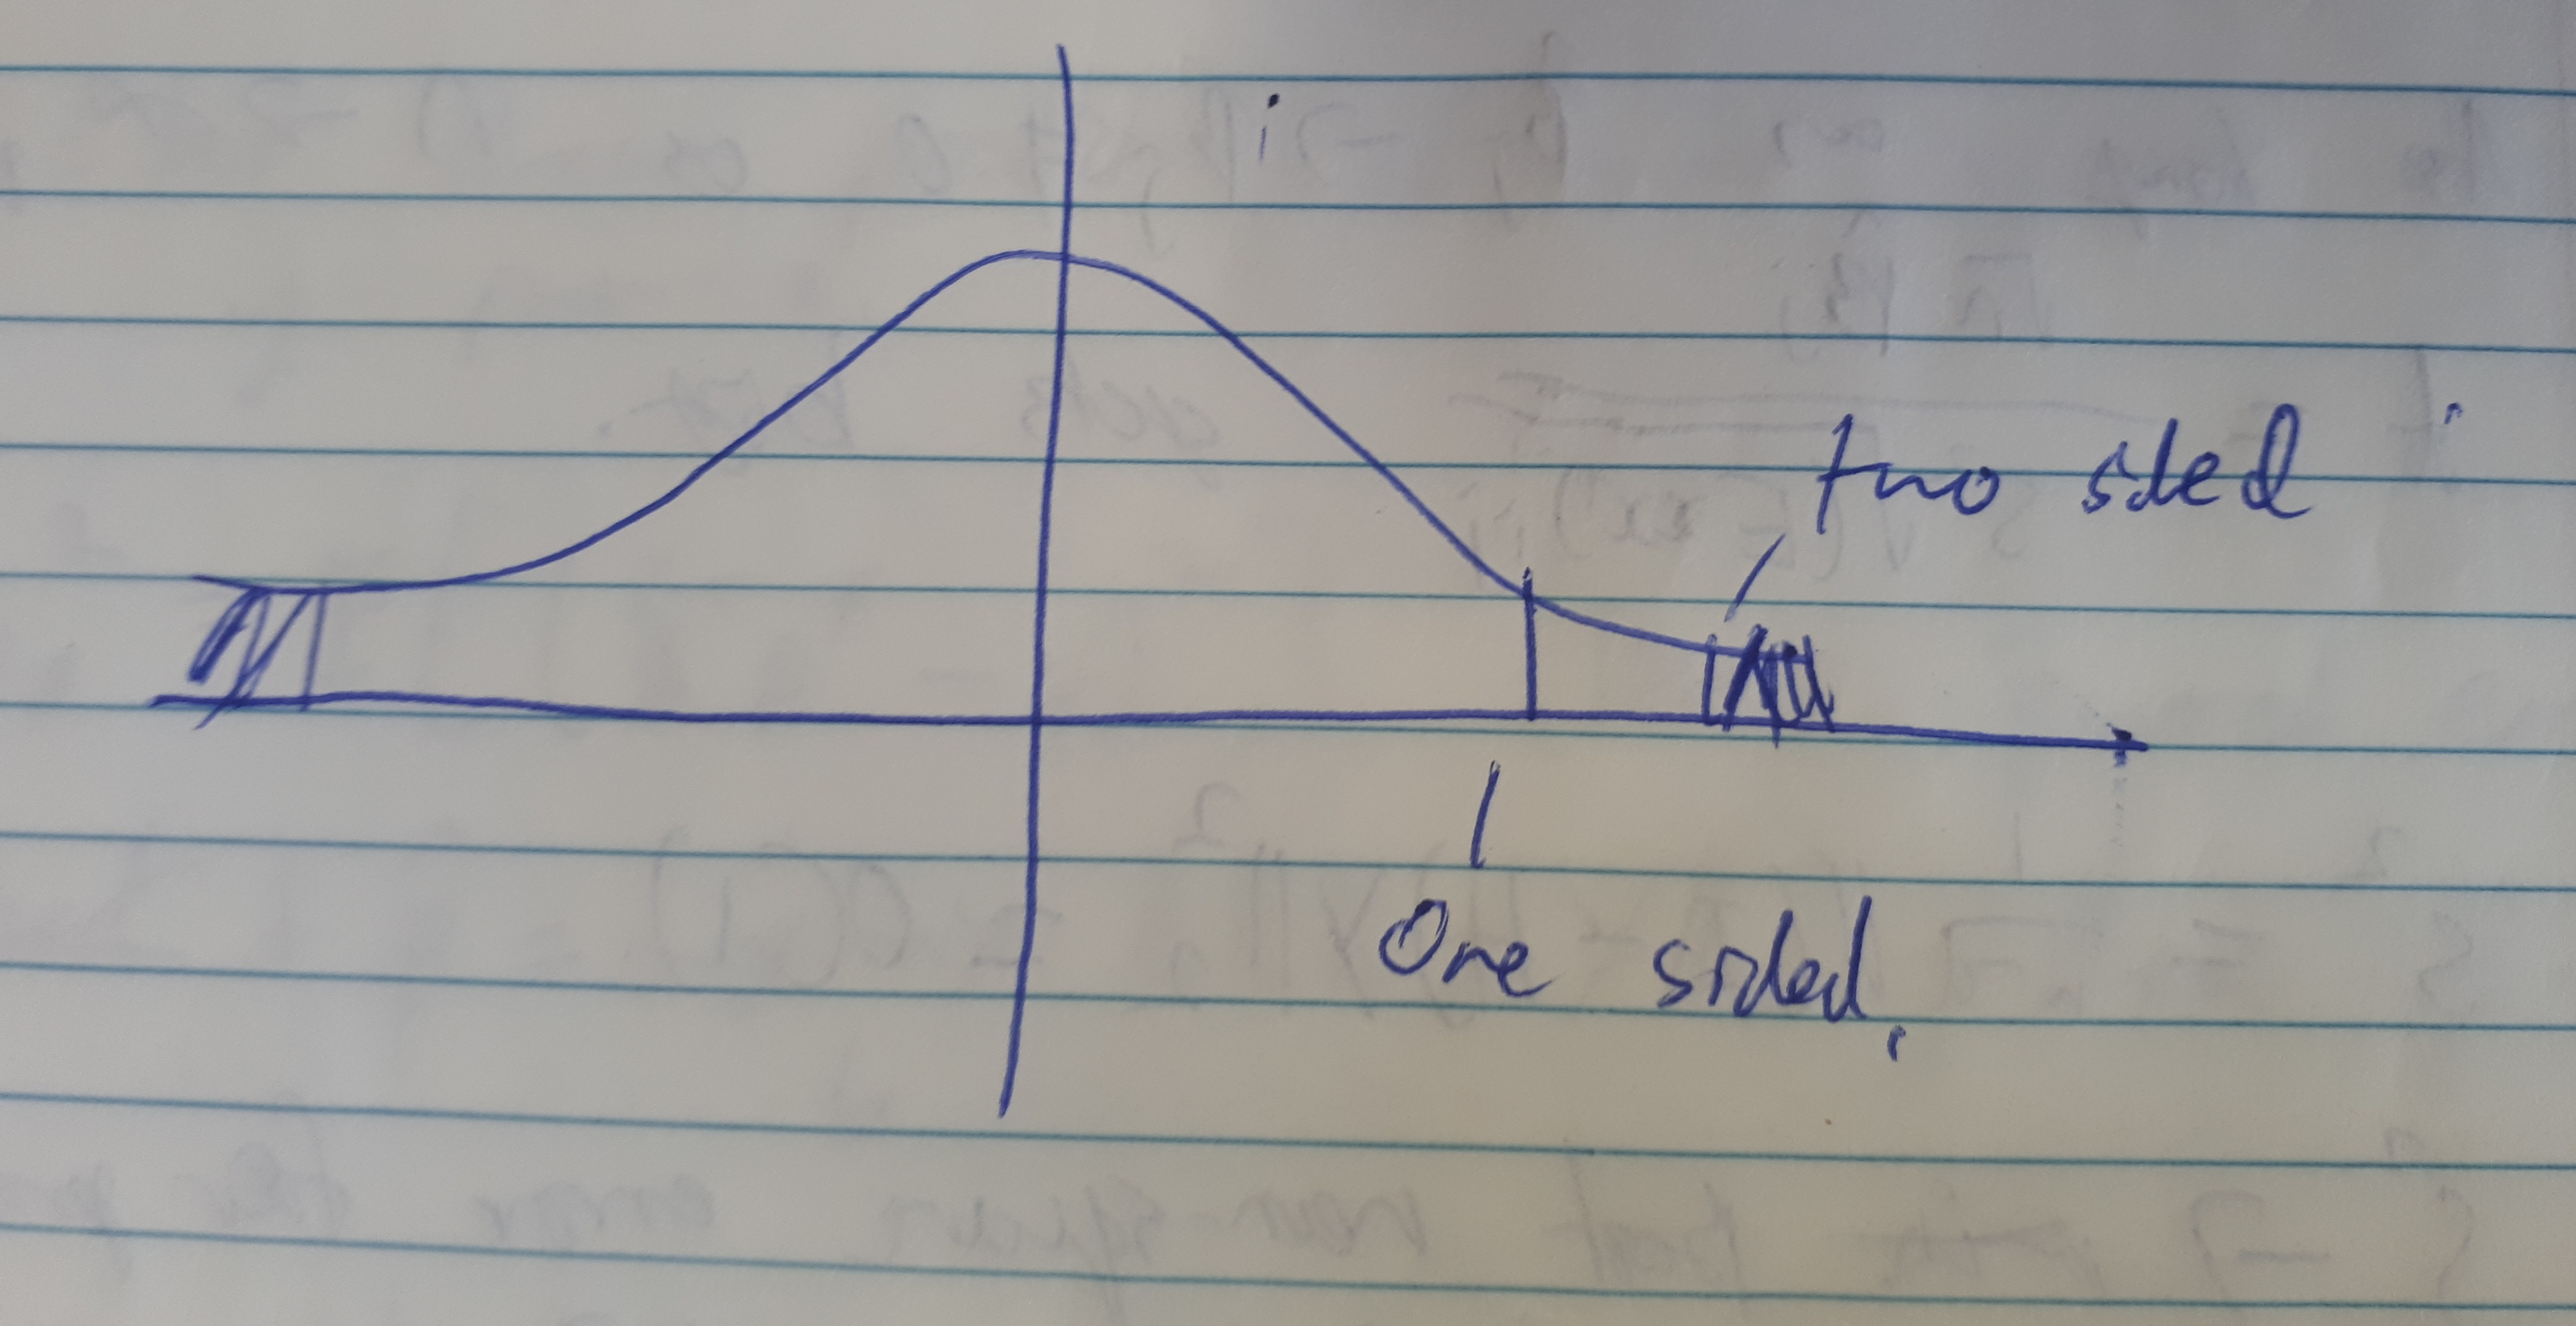
\includegraphics[width = \textwidth/2]{10_05_P01.jpg}
\end{center}
We can ask what happens to our $t$-statistic as $n\to \infty$ (we get more and more data observations). Suppose that $c = e_j$ and so $c^T\beta = \beta_j$. Then our t-statistic is
\[\frac{\wh{\beta}_j-\beta_j}{S^2\sqrt{(X^TX)^{-1}_{jj}}}. \]
How it changes with $n$ shows the difference between pratical and statistical significance. Note
\[X^TX = \sum_{i=1}^n x_ix_i^T \approx n \E[xx^T], \]
and thus
\[(X^TX)^{-1} = \frac{1}{n}\left(\frac{1}{n}X^TX\right)^{-1} \approx \frac{1}{n}(\E[xx^T])^{-1}. \]
Thus $(X^TX)^{-1}$ gets smaller as $n$ grows. Thus our t-statistic is approximately 
\[t=\frac{\wh{\beta}_j-\beta_j}{S^2\sqrt{
    \frac{1}{n}\left(\E xx^T\right)^{-1}_{jj}}}= \frac{\sqrt{n}(\wh{\beta}_j-\beta_j)}{S^2\sqrt{
    \left(\E xx^T\right)^{-1}_{jj}}}.\]
As long as $\wh{\beta}_j \to \beta_j \neq 0$ as $n \to \infty$, then 
\[t = \frac{\sqrt{n}\wh{\beta}_j}{S^2\sqrt{(\E xx^T)^{-1}_{jj}}}, \]
gets big. Note that $S^2$ stays roughly constant with $n$ since
\[S^2 = \frac{1}{n-d}\norm{(I-H)Y}_2^2 = O(1). \]
Also $S^2$ converges to the best mean-square error for the problem. Note that \[\wh{\beta}_j \to \text{argmin}_{b}\E[(x^Tb-y)^2],\] 
and thus argmin is not 0 in any real world problems.

Thus with enough data we can reject any null hypothesis based on the t-test. This is because if our null if $\beta_j = 0$, then the statistic we compute is
\[t=\frac{\wh{\beta}_j}{S^2 \sqrt{(X^TX)_{jj}}} \approx \frac{\sqrt{n}\wh{\beta}_j}{S^2\sqrt{
    \left(\E xx^T\right)^{-1}_{jj}}}. \]

One implication of this is that models should become more sophisticated as our amount of data grows. This may mean getting new features or having less specific assumptions on the errors.

Let's do the same calculations for $n \to \infty$ with a bit more rigor and detail. Define
\[\beta^* = \text{argmin}_b \E[(x^Tb-y)^2], \]
so $\beta^* $ is the best linear predictor under square error of $y$ from $x$. Also define
\[S^2_* = \E[(x^T\beta^* -y)^2],\]
the best possible square error. We can make the following assertions if $\wh{\beta} = \text{argmin}_b \norm{X b -Y}_2^2$, then $\wh{\beta} \to \beta^*$ and if $S^2 = \frac{1}{n-d}\norm{X\wh{\beta}-Y}_2^2$, then $S^2 \to S_*^2$ and $\frac{1}{n} \sum_{i=1}^n x_ix_i^T \to C := \E[xx^T] \succ 0$. Then the test statistic under the assumed null $H_0 :\beta_j = 0$, satisfies
\begin{IEEEeqnarray*}{rCl}
    t&:=&\frac{\wh{\beta}_j}{S^2\sqrt{(X^TX)^{-1}_{jj}}}\\
    &=&\frac{\sqrt{n} \beta_j^*}{S_*^2\sqrt{(C^{-1})_{jj}}}(1+o(1))\\
    &=&\text{sgn}(\beta_j^*)\cdot \infty.
\end{IEEEeqnarray*}
Thus even if $\beta_j^*$ is very very close to 0, we will reject the null if we have enough data. 

Note that at a fixed significance level, the thresholds don't change very much with $n$ since the $T$ distribution converges to a standard normal as $n$ goes to infinity.

The upshot is that pratical significance does not equal statistical significance.
\subsection{Using R}
In R if you run ``\texttt{L <- lm()}'' and then run ``\texttt{summary(L)}'', then you will get T-statistics for each regressor. These are the T-statistics we have been talking about. 

These are the $p$-values for $\beta_j$ \underline{controlling for} $\{\beta_0,\ldots, \beta_d\} \setminus \{\beta_j\}$.
\subsection{F-tests}

Recall the F-distribution. If $U \sim \chi^2_d$ and $V \sim \chi^2_n$ and $U \ind V$, then 
\[\frac{\frac{1}{d}U}{\frac{1}{n}V} \sim F_{d,n}, \]
we say that $\frac{\frac{1}{d}U}{\frac{1}{n}V}$ has an F-distribution with $n$ degrees of freedom on top and $d$ degrees of freedom on the bottom. 

Tests based on F-statistics are more directly tied to how well our model fits the data.

\begin{thrm}
    Assume we have a linear model $Y = X\beta + \varepsilon$, $\varepsilon \sim \Na(0, \sigma^2 I)$. Let $C \in \R^{d \times r}$ with $r \le d$ ($C$ is tall) and suppose $C$ has rank $r$. Then 
    \begin{equation}\label{F-dist}
        \frac{\frac{1}{r}\left(\left(C^T(\wh{\beta}-\beta)\right)^T\left(C^T(X^TX)^{-1}C\right)^{-1}\left(C^T(\wh{\beta}-\beta)\right)\right)}{S^2} \sim F_{r,n-d},
    \end{equation}
    where, as before, $S^2 = \frac{1}{n-d}\sum_{r=1}^n (y_i-x_i^T\wh{\beta})^2.$
\end{thrm}
\begin{ex}
    If $c = e_j$, then $r=1$ and 
    \[\frac{1}{S^2}\frac{(\wh{\beta}_j-\beta_j)^2}{[(X^TX)^{-1}]_{jj}} \sim F_1,n-d. \]
    This tests if $\beta_j \neq 0$ or if feature $j$ should be included in our model. We would reject the null $\beta_j = 0$ if the above statistic if large.
\end{ex}
\begin{proof}
    \emph{[Of equation \eqref{F-dist}]} By our main independence result
    \[C^T(\wh{\beta}-\beta) \sim \Na(0, \sigma^2 C^T(X^TX)^{-1}C), \]
    and $S^2 = \frac{1}{n-d}\norm{(I-H)Y}_2^2 = \frac{1}{n-d}\norm{(I-H)\varepsilon}_2^2 \sim \frac{\sigma^2}{n-d} \chi^2_{n-d}$ since $I-H$ has rank $n-d$. Also $c^T(\wh{\beta}-\beta)$ is independent of $S^2$.

    Recall that we have seen if $w \sim \Na(0,B)$, then $B^{-1/2}w \sim \Na(0,I)$ and thus $wB^{-1}w \sim \chi^2_{\text{rank}(B)}$. Thus 
    \begin{IEEEeqnarray*}{rCl}
        &&\left(\left(C^T(\wh{\beta}-\beta)\right)^T\left(C^T(X^TX)^{-1}C\right)^{-1}\left(C^T(\wh{\beta}-\beta)\right)\right)\\
        &=&\sigma^2 \sum_{i=1}^r z_i^2 \quad \text{where } z_i \sim \Na(0,1)\\
        &\sim& \sigma^2 \chi^2_r.
    \end{IEEEeqnarray*}
    Thus the ratio in equation \eqref{F-dist} equals
    \[\frac{\frac{\sigma^2}{r}\chi^2_r}{\frac{\sigma^2}{n-d}\chi^2_{n-d}} = \frac{\frac{1}{r}\chi^2_r}{\frac{1}{n-d}\chi^2_{n-d}} \sim F_{n,d}. \]
\end{proof}
\subsection{Testing submodels}
Question: is there a submodel in $Y=X\beta +\varepsilon$ that is just as good as the full model.

Suppose we have an $X_0$ such that $\range(X_0)\subseteq \range(X)$ and we assume that $Y = X_0\gamma + \varepsilon$. For example we may have $X = [1, x^{(1)},\ldots, x^{(d)}]$ and $X_0 = [1, x^{(1)},\ldots, x^{(d-k)}]$. 

Assuming that the linear model $Y=X_0\gamma + \varepsilon$ is ``good enough'', define
\begin{IEEEeqnarray*}{rCl}
    H_0&=&X_0(X_0^TX_0)^{-1}X_0^T,\\
    H&=&X(X^TX)^{-1}X^T
\end{IEEEeqnarray*}
That is, $H_0$ projects onto $\range(X_0)$ and $H$ projects onto $\range(X)$. Note that $H_0$ is no longer notation for the null hypothesis but rather for a matrix. 

Note that $H \succeq H_0$ i.e. $H-H_0 \succeq 0$. This is because $H_0 =\sum_{i=1}^r u_iu_i^T$ and $H=\sum_{i=1}^r u_iu_i^T+\sum_{i=r+1}^d u_iu_i^T$ where $\{u_i\}$ are orthonormal vectors. Then $H-H_0 = \sum_{i=r+1}^d u_iu_i^T$. We can also think geometrically. Since $H_0$ projects onto a subspace of $H$, we can conclude that $H-H_0$ projects onto the subspace of vectors in $\range(X)$ that are orthogonal to $\range(X_0)$. Since $H-H_0$ is a projection, we have $H-H_0 \succeq 0$. Note $HH_0 = H_0 = H_0H$ and $H_0 \perp H-H_0$. This last point is because $H-H_0$ is the part of the full model that is orthogonal to the submodel. 

\begin{prop}
    Assume $Y = X_0\gamma + \varepsilon$, $\varepsilon\sim \Na(0, \sigma^2 I)$ and $\text{rank}(X_0) = d-r < d = \text{rank}(X)$. Then 
    \begin{equation}\label{F2}
        \frac{\frac{1}{r}\norm{(H-H_0)Y_2^2}}{\frac{1}{n-d}\norm{(I-H)Y}_2^2}\sim F_{r,n-d} 
    \end{equation}
\end{prop}
We have the following intepretation. Let $\wh{Y}=HY=$ predictions using the full model and $\wh{Y}^{sub} = H_0Y=$ predictions using the submodel. Then $SS_{full} = \sum_{i=1}^n(y_i-\wh{y}_i)^2 = \norm{(I-H)Y}_2^2$ and $SS_{sub} = \sum_{i=1}^n(y_i-\wh{y}_i^{sub})^2 = \norm{(I-H_0)Y}_2^2$. Thus
\begin{IEEEeqnarray*}{rCl}
    SS_{extra}&=&SS_{sub}-SS_{extra}\\
    &=&\norm{(I-H_0)Y}_2^2-\norm{(I-H_0)Y}_2^2\\
    &=&-Y^TH_0Y+Y^THY\\
    &=&Y^T(H-H_0)Y\\
    &=&\norm{(H-H_0)Y}_2^2.
\end{IEEEeqnarray*}
Thus if the ratio in equation \eqref{F2} is very large we should use the full model. If it is very small we will use the submodel. We will now prove \eqref{F2}.
\begin{proof}
    \begin{IEEEeqnarray*}{rCl}
        (H-H_0)Y&=&(H-H_0)(X_0\gamma + \varepsilon)\\
        &=&(H-H_0)\varepsilon \sim N(0,\sigma^2(H-H_0))
    \end{IEEEeqnarray*}
    and
    \begin{IEEEeqnarray*}{rCl}
        (I-H)Y&=&(I-H)(X_0\gamma + \varepsilon)\\
        &=&(I-H)\varepsilon \sim N(0,\sigma^2(I-H))
    \end{IEEEeqnarray*}
    We also have $(H-H_0)Y \ind (I-H)Y$ since
    \begin{IEEEeqnarray*}{rCl}
        (H-H_0)(I-H)&=&H-H_0-H^2+H_0H\\
        &=&H-H_0-H+H_0\\
        &=&0.
    \end{IEEEeqnarray*}
    Since $\text{rank}(I-H) =n-d$ and $\text{rank}(H-H_0)=d-(d-r)=r$, the result follows.
\end{proof}
The intuition is that $(I-H)Y$ is outside the full model and $(H-H_0)Y$ is the part of the full model orthogonal to the sub model. Thus $(I-H)Y$ are $(H-H_0)Y$ are independent.

One more comment. In ``science'' when people report F-tests they are testing $X_0 = [1]$ against $X = [1, x^{(1)},\ldots, x^{(d)}]$. What does rejecting the null mean in this case? Implicit in our derivation of the test is the assumption that the full model is the truth. The rejecting the null means we are not in the world where the full model and the sub model are both true. We may in the world were the full model is true and the sub model is false or we may be in the world were \underline{both are false}. 
\end{document}